%!TEX root = ../../adrien_gomar_phd.tex

\chapter*{Conclusion}

\section*{Summary of the results}
\label{sec:perspectives}

The industrial design of turbomachinery, 
and by extension contra-rotating
open rotors, is usually based on steady flow analysis. 
However, this approach finds its limits 
when unsteady phenomena become dominant. This is the case of 
contra-rotating open rotors where the interaction between the
two rotors is of prior importance or when
aeroelastic effects have to be considered. In such a
context, engineers need now tools to account for these effects as
early as possible in the design cycle. With the growth of
computational power, unsteady computations are entering industrial
practice, but the associated restitution time remains an obstacle for
daily basis applications. For this reason, efficient
unsteady approaches are receiving a lot of attention. 

Fourier-based time methods rely on direct and inverse Fourier transforms
to turn the time-marching problem into the coupled resolution of several
mathematically steady problems representing snapshots of the unsteady
solution. In the turbomachinery community, this approach has
proven to be very efficient, yielding up to two orders of
magnitude computational time reduction compared to classical
time-marching simulations.

\subsection*{On the multi-frequential harmonic balance approach}

When unsteadiness is related to a single frequency and its
harmonics, Fourier analysis leads to a natural choice for time instances:
they are evenly spaced over the period. In this case, the mathematical
problem is numerically well-posed, meaning that the conditioning of
the operators ensures the convergence of the approach.
In opposite, when several arbitrary frequencies are 
considered, as for instance contra-rotating open rotor
aeroelasticity, the multi-frequential harmonic balance approach
is required.

In \hyperref[cha:limitations_condition_number]{\emph{Chapter~5}},
we demonstrated that the time sampling has a major effect on the
stability of the multi-frequential harmonic balance 
method, due to the condition number of the Fourier
transform matrix. One way to tackle this issue, 
is to consider a non-uniform time sampling
along with an algorithm to properly choose them
as proposed by \citet{ThesisGuedeney}
The APFT algorithm, developed
by \citet{Kundert1988} and implemented by 
\citet{ThesisGuedeney}, is shown to improve the
Fourier matrix orthogonality in order to 
reduce its condition number, while
the OPT algorithm, developed in the current work, 
directly minimizes the condition number thanks to a
gradient-based optimization method. This last has proven to
give a condition number almost unity for any input frequencies,
thus alleviating the stability issues attributed to 
the condition number.

\subsection*{On the convergence of Fourier-based time methods}

The accuracy and efficiency of Fourier-based time methods 
used to solve periodic unsteady problems depends on the number of harmonics
chosen to represent the frequency content of the time signal.
In this work we investigate the accuracy and convergence properties 
of Fourier-based time integration methods. The convergence rate 
of these methods, in terms of harmonics required to describe the solution 
with a given level of accuracy, depends on the spectral content of the 
solution itself: Fourier-based time methods are particularly efficient 
for flow problems characterized by a narrow Fourier 
spectrum. Starting from this remark, we try to define a relevant 
indicator of solution regularity in the specific case of turbomachinery 
flows, which represent one of the main applications of Fourier-based 
time methods in Fluid Mechanics.
To this aim, we show that main source of unsteadiness in 
turbomachinery flows is due to the relative motion of wakes 
generated by a given blade row with respect to the downstream row. 
Statistically speaking, the passing wakes are seen by the downstream 
row as an azimuthally advected periodic Gaussian pulse, 
characterized by its relative thickness compared to the pitch 
in between two subsequent blades and by the velocity deficit 
associated to it. We show that the narrower the wake, the larger 
its Fourier spectrum, and the slower the convergence of Fourier-based time methods.
In order to achieve a priori estimates of the number of 
harmonics required to accurately solve a given turbomachinery 
problem, we introduce two error measures based on the relative 
thickness of the passing wakes. It is shown that, for practical 
purposes, these can be preliminarily estimated by running a 
companion steady simulation of the turbomachinery stage. The 
steady simulation is post-processed to extract information about 
the spanwise distribution of wake thickness, and an error criterion 
is used to estimate the number of harmonics required to resolve 99\% 
of the energy content associated to the velocity signal. The 
preliminary step has a negligible cost compared to the overall 
simulation, since the steady computation is used to initialize 
the unsteady run, and extraction of wake characteristics takes 
less than a minute on a single processor. 

The proposed methodology represents an efficient and reliable 
operational tool to guide the choice of the number of harmonics 
for a given turbomachinery problem, and to evaluate beforehand the 
interest of applying or not a Fourier-based time integration scheme 
instead of a classical time-marching scheme.


The HB approach for aeroelastic damping calculation, derived for
periodic problems where the period is known \emph{a priori}, has been
presented. 
The phase-lagged boundary conditions are then purely derived in the
time-domain, which is expected to be more computationally efficient and 
easier to implement. 
Finally, the proposed method has been
validated on the $11^{th}$ standard configuration and applied to an
industrial case. The results show that the HB approach provides local
and global results close to the reference DTS scheme with only three
instances (one harmonic) in the time period.  At the cost of a memory
increase (roughly equal to the number of instances used in the HB
simulations), the computational saving is about a factor 3 to 10,
depending on the case considered, the operating point and the value of
the IBPA. For the $11^{th}$ standard configuration, the results are
in good agreement with the experimental data and with the results
found in the literature.  For the fan case considered in the present
study, the critical damping is well predicted at the nominal point.
In practice, the HB method is a good candidate for fast preliminary
design investigations, that could be complemented by more advanced
studies.

Les résultats obtenus avec l’approche HBT sont concluants. Les courbes d’amortissement obtenues sont proches des courbes présentent dans la littérature (forme en "S"). Le post-traitement de l’amor- tissement surfacique a permit de mieux comprendre l’origine de l’amortissement intégré. L’approche mise en place est maintenant robuste, le choix des instants et des fréquences et le post-traitement de tels calculs sont des points maîtrisés.

\section*{Future work}
\label{sec:perspectives}

Another point of interest is the shape optimization of industrial
turbomachinery to improve their efficiency. Among other optimization approaches, 
gradient based optimization
techniques using adjoint calculations have become popular for the
design of complex systems parameterized by a large number of design variables
since the pioneering work of Jameson~\cite{jameson88}. However,
both computational cost and technical difficulties can be prohibitive for
unsteady flows: the adjoint system has to be solved in a reverse way and
Navier-Stokes solutions have to be stored during the iterative process.
These problems remain for periodic flows with classical time marching 
integration schemes. With the considered harmonic methods, computing
sensitivities is much simpler since the residuals to be derived with 
respect to the state variables and the mesh nodes coordinates are 
similar to RANS equations of which adjoint state is classicaly computed. 
As a consequence, the
computational cost for adjoint sensitivities of such flows is affordable
and the overall complexity is finally moderate. Duta et al.~\cite{Duta01}
have used this technique in the context of aeroelastic turbomachinery
design and a wide range of potential applications for the HB method is now
opened.

\begin{figure}[htp]
  \centering
  \subfigure[2F]{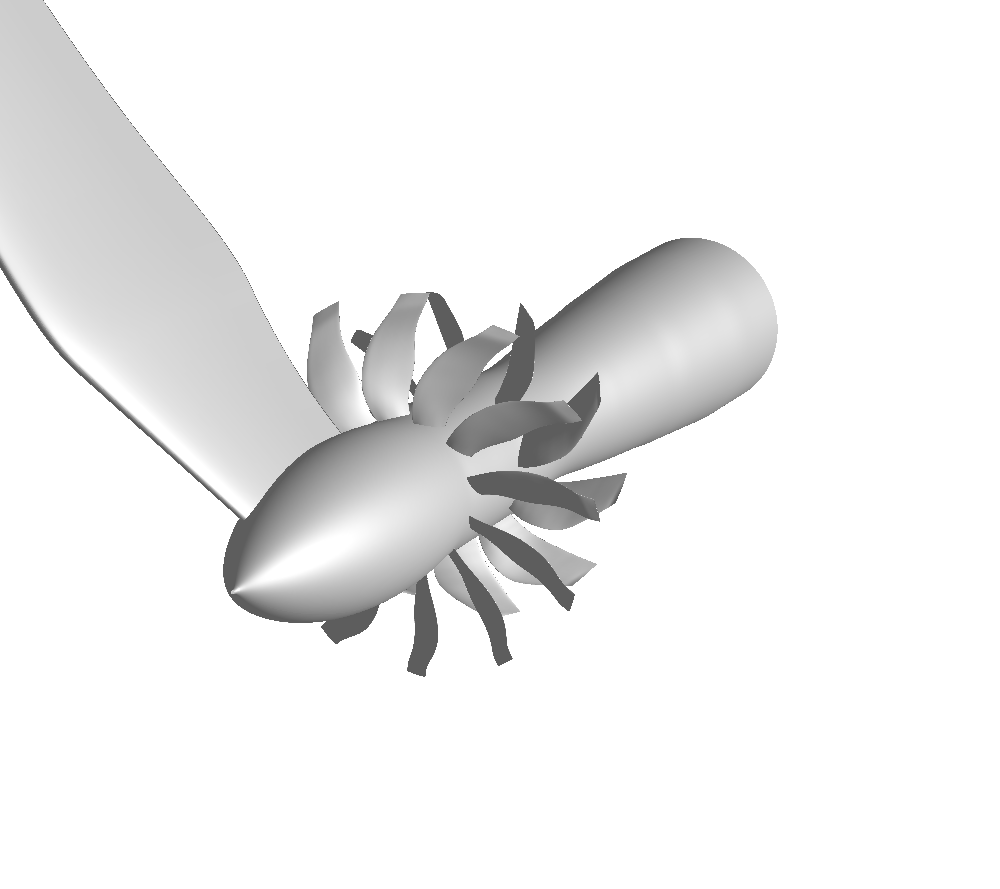
\includegraphics[width=.4\textwidth]{HERA3_INSTALLED_wall.png}}
  \subfigure[1T]{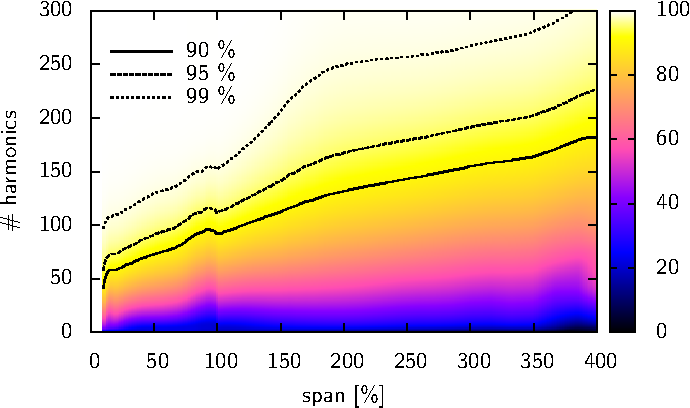
\includegraphics[width=0.40\textwidth]{HERA3_INSTALLED_RANS_SPECTRUM_PPT.pdf}}
  \caption{Low-speed isolated configuration: structural modes considered.}
  \label{fig:hera3_perspectives}
\end{figure}
